\begin{figure}[ht!]
%
% \begin{center}
% \centering
\begin{subfigure}[t]{0.23\textwidth}
% \centering
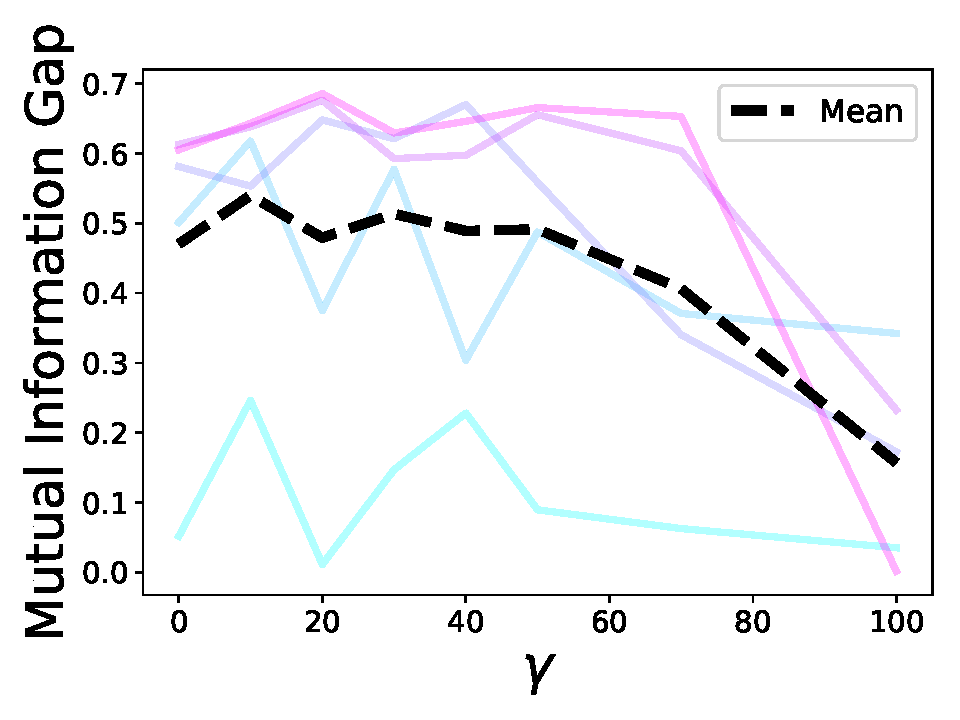
\includegraphics[width=\textwidth]{mig_gamma_beta_sens_low_lines.pdf}
\caption{Colour is $\alpha$}
\label{fig:dsprites-mig-lines-low-alpha}
\end{subfigure}
%
\hfill
%
\begin{subfigure}[t]{0.23\textwidth}
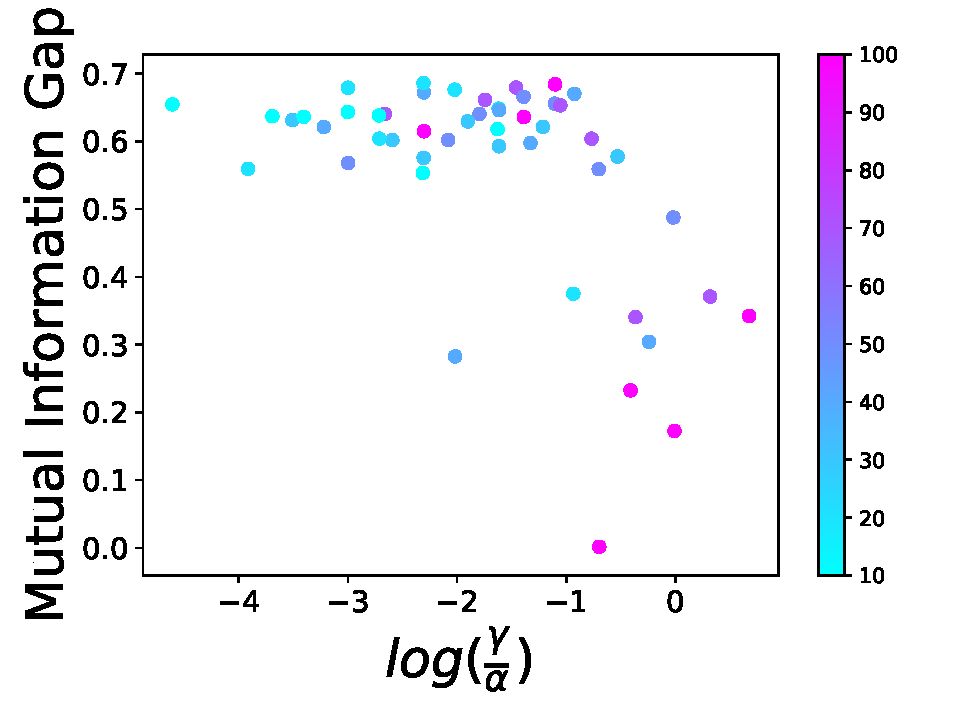
\includegraphics[width=\textwidth]{mig_gamma_betasens_ratio.pdf}
\caption{Colour is $\gamma$}
\label{fig:dsprites-mig-ratio}
\end{subfigure}


\caption{
    Mutual Information Gap (MIG) for various $(\alpha, \gamma)$ settings of the FFVAE. 
    In Fig. \ref{fig:dsprites-mig-lines-low-alpha}, each line is a different value of
    $\alpha \in [0, 50, 100, 150, 200]$, with brighter colours indicating larger values of $\alpha$.
    In Fig. \ref{fig:dsprites-mig-ratio}, all combinations with $\alpha, \gamma > 0$ are shown.
    Models trained on DspritesUnfair, MIG calculated on Dsprites.
    Higher MIG is better.
    Black dashed line indicates mean (outliers excluded).
    $\alpha = 0$ is equivalent to the FactorVAE.
    }
    \label{fig:dsprites-mig-appendix}
% \end{center}
% \vskip -0.2in
\end{figure}
